\documentclass[border=10pt]{standalone}
\usepackage{tikz}
\usetikzlibrary{positioning}

\tikzset{
  layer/.style = {rectangle, draw, thick, minimum width=6cm,
                  minimum height=1.2cm, align=center, inner sep=6pt},
  ref/.style   = {font=\small}
}

\begin{document}
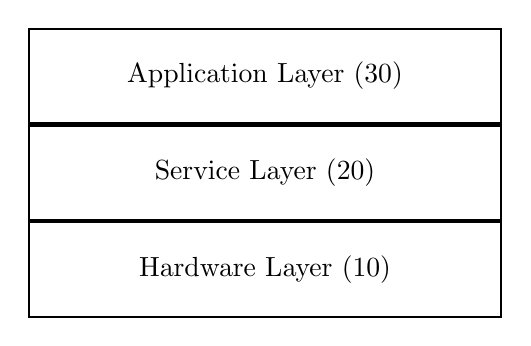
\begin{tikzpicture}[node distance=0cm]
  \node (A) [layer] {Application Layer (30)};
  \node (B) [layer, below=of A] {Service Layer (20)};
  \node (C) [layer, below=of B] {Hardware Layer (10)};
\end{tikzpicture}
\end{document}
